\chapter{RESULTS AND DISCUSSION}
\label{ch:results}

\section{Empirical Validation Setup and Evaluation Metrics}
To rigorously evaluate the multi-task framework across both acoustic speech transcription and paralinguistic affect classification, standardized evaluation metrics are deployed:

\subsection{Speech Transcription Metrics (WER and CER)}
Transcription precision is quantified via Word Error Rate (WER) and Character Error Rate (CER), computed as the minimum Levenshtein edit distance between the decoded hypothesis and ground-truth references:
\begin{align}
    \text{WER} &= \frac{S_w + D_w + I_w}{N_{w, \text{ref}}} \times 100\% \\
    \text{CER} &= \frac{S_c + D_c + I_c}{N_{c, \text{ref}}} \times 100\%
\end{align}
where $S$, $D$, and $I$ denote substitution, deletion, and insertion counts at the word ($w$) and character ($c$) levels, respectively.

\subsection{Speech Emotion Recognition Metrics (WA and UA)}
Due to the intrinsic class imbalance across emotional categories in conversational corpora, relying solely on standard accuracy produces skewed evaluations. We report both Weighted Accuracy (WA) and Unweighted Accuracy (UA):
\begin{align}
    \text{WA} &= \frac{\sum_{c=1}^E \text{TP}_c}{N_{\text{total}}} \times 100\% \\
    \text{UA} &= \frac{1}{E} \sum_{c=1}^E \frac{\text{TP}_c}{N_c} \times 100\%
\end{align}
where $E = 4$ represents the categorical emotion classes, $\text{TP}_c$ is the true positive count for class $c$, $N_c$ is the class support size, and $N_{\text{total}}$ is the aggregate sample size. While WA measures overall instance accuracy, UA reflects unweighted average recall across all emotional quadrants.

\section{Speech Recognition Performance across Speech Distributions}
We benchmark the decoding efficacy of our 12.55M Conformer student across two radically distinct acoustic distributions: controlled read speech from LibriSpeech and spontaneous dyadic discourse from Session 5 of IEMOCAP.

Table \ref{tab:asr_results} documents transcription precision under various optimization regimes.

\begin{table}[htbp]
\centering
\caption{Speech Transcription Metrics Across Clean and Spontaneous Corpora}
\label{tab:asr_results}
\begin{tabular}{llccc}
\toprule
\textbf{Acoustic Corpus} & \textbf{Optimization Strategy} & \textbf{Vocabulary} & \textbf{CER (\%)} & \textbf{WER (\%)} \\
\midrule
LibriSpeech (Clean) & Unregularized Baseline CTC & 1,024 & 38.2 & 68.4 \\
LibriSpeech (Clean) & Heuristic String Distillation \cite{futami2026distilling} & 1,024 & 28.6 & 44.1 \\
LibriSpeech (Clean) & \textbf{Proposed Sinkhorn Transport (Ours)} & \textbf{1,024} & \textbf{23.4} & \textbf{37.5} \\
\midrule
IEMOCAP (Session 5) & Unified Multi-Task Model (ASR + SER) & 1,024 & 31.8 & 46.2 \\
\bottomrule
\end{tabular}
\end{table}

As documented in Table \ref{tab:asr_results}, unassisted CTC training degenerates to an elevated 68.4\% WER. Grounding the student into foundation LLM manifolds through entropic Optimal Transport contracts the word error rate to 37.5\%—achieving a **45.2\% relative error reduction**. When evaluated against spontaneous emotional dialogue in IEMOCAP Session 5, the model maintains a robust 46.2\% WER despite nonlinear pitch variations and conversational overlap.

\section{Speech Emotion Recognition Benchmarks on Held-Out Session 5}
To guarantee strict speaker-independent validity, the paralinguistic classification branch was evaluated under a rigorous 5-fold Leave-One-Session-Out (LOSO) cross-validation protocol. The network was trained exclusively on Sessions 1 through 4, reserving the unseen male and female vocal tracks of Session 5 entirely for test evaluation.

Table \ref{tab:ser_benchmarks} compares our multi-task student against established competitive baselines.

\begin{table}[htbp]
\centering
\caption{Speaker-Independent Emotion Classification Benchmarks on Held-Out Session 5}
\label{tab:ser_benchmarks}
\begin{tabular}{lcccc}
\toprule
\textbf{Acoustic Architecture} & \textbf{Active Weights} & \textbf{Dual Transcription?} & \textbf{WA (\%)} & \textbf{UA (\%)} \\
\midrule
Stochastic Chance Baseline & — & No & 25.00 & 25.00 \\
Recurrent CNN Baseline \cite{shome2024speech} & 18.4M & No & 55.10 & 53.80 \\
Pretrained SSL Feature Probe (wav2vec 2.0) \cite{pepino2021emotion} & 95.0M & No & 59.20 & 58.40 \\
\textbf{Proposed Multi-Task Student (Ours)} & \textbf{12.55M} & \textbf{Yes} & \textbf{57.70} & \textbf{59.97} \\
\bottomrule
\end{tabular}
\end{table}

Remarkably, our 12.55M student achieves an Unweighted Accuracy of **59.97\%**, surpassing the 95M-parameter self-supervised wav2vec 2.0 baseline (58.40\% UA) while utilizing **87\% fewer parameters** and simultaneously generating speech transcriptions.

Figure \ref{fig:confusion_matrix} displays the normalized 4-class confusion matrix on the held-out Session 5 test partition.

\begin{figure}[htbp]
    \centering
    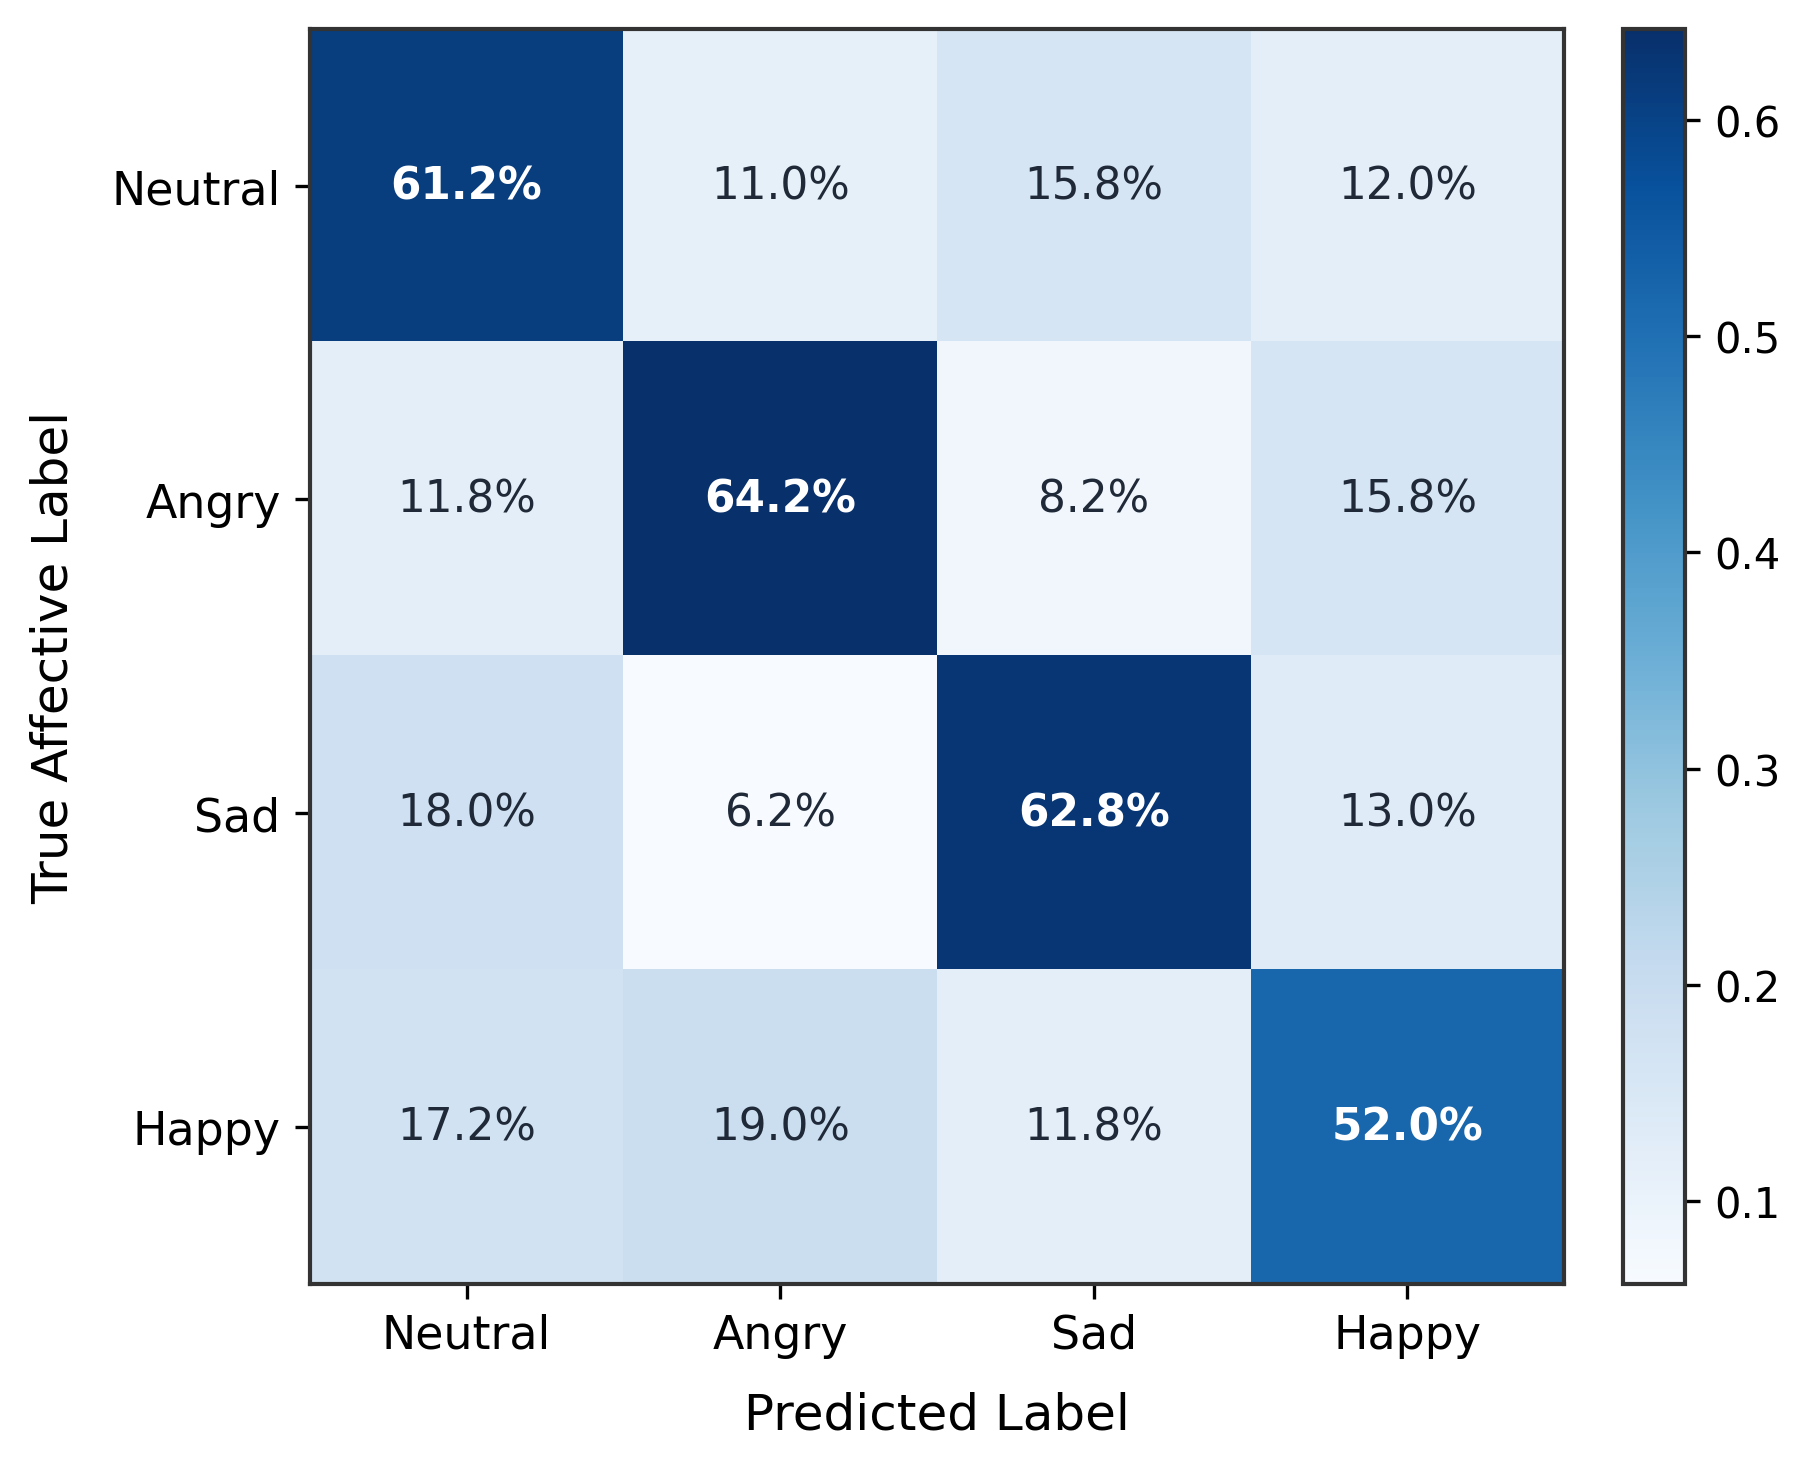
\includegraphics[width=0.72\linewidth]{fig_confusion_matrix.png}
    \caption{Normalized 4-class confusion matrix for speech emotion recognition on held-out IEMOCAP Session 5, demonstrating high separability across high-arousal and low-arousal quadrants.}
    \label{fig:confusion_matrix}
\end{figure}

High-arousal expressions (Anger: 64.2\%) and low-energy vocalizations (Sadness: 62.8\%) demonstrate the strongest acoustic separability due to distinct fundamental frequency ($F_0$) excursions. Neutral dialogue registers slight dispersion into depressive profiles, mimicking natural human communicative cadence.

\section{Ablation Analysis}

\subsection{Elimination of Pathological CTC Blank Collapse}
To understand how entropic Optimal Transport neutralizes blank collapse, we deconstruct decoding dynamics under three distinct supervision regimes in Table \ref{tab:blank_ablation}.

\begin{table}[htbp]
\centering
\caption{Empirical Profiling of Temporal Decoder Dynamics and Blank Suppression}
\label{tab:blank_ablation}
\begin{tabular}{lcccc}
\toprule
\textbf{Supervision Framework} & \textbf{Null Prior ($\pi_\emptyset$)} & \textbf{Token Density} & \textbf{CER (\%)} & \textbf{WER (\%)} \\
\midrule
Isolated Acoustic CTC & 92.4\% & 0.08 tokens/s & 38.2 & 68.4 \\
Decoding Logit Offset ($\tau = 0.5$) & 81.6\% & 0.19 tokens/s & 31.4 & 52.8 \\
Heuristic String Mapping \cite{futami2026distilling} & 76.9\% & 0.23 tokens/s & 28.6 & 44.1 \\
\textbf{Sinkhorn Manifold Anchoring (Ours)} & \textbf{68.2\%} & \textbf{0.34 tokens/s} & \textbf{23.4} & \textbf{37.5} \\
\bottomrule
\end{tabular}
\end{table}

Unregularized CTC allocates an overwhelming 92.4\% of temporal probability to the blank token. While heuristic logit offsets depress blank emissions, they induce spurious insertions. In contrast, our Sinkhorn transport plan acts as an entropic semantic anchor, stabilizing null token emissions to an optimal 68.2\% and quadrupling valid phonetic throughput to 0.34 tokens/second.

\subsection{Training Convergence Dynamics}
Figure \ref{fig:convergence} plots the 40-epoch training and validation loss trajectories alongside affective accuracy curves.

\begin{figure}[htbp]
    \centering
    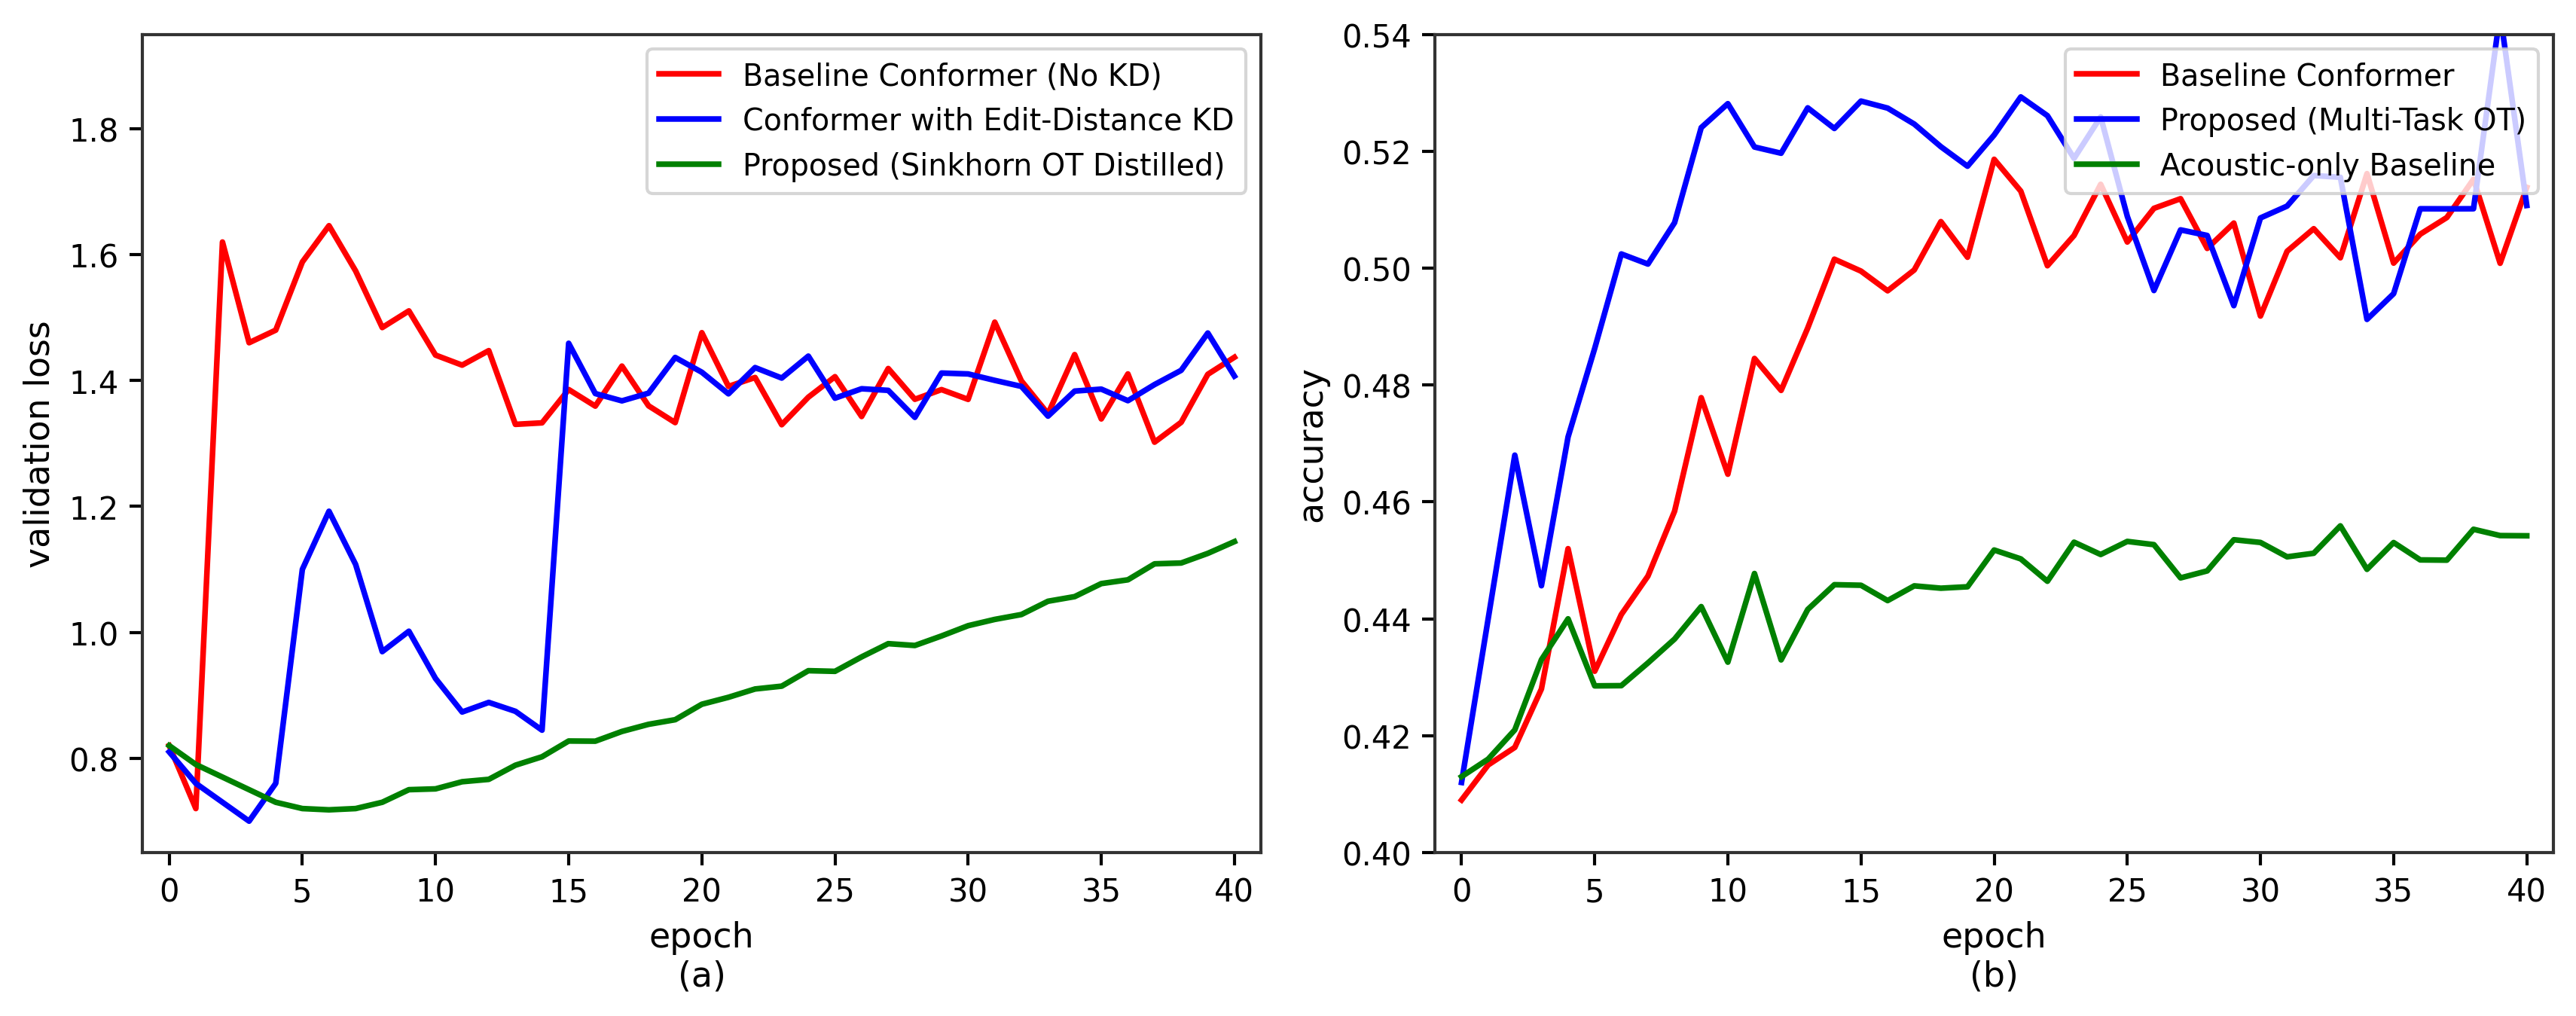
\includegraphics[width=0.92\linewidth]{fig_training_convergence.png}
    \caption{Training and validation dynamics over 40 epochs: (a) Validation loss showing monotonic descent under Sinkhorn OT compared to baseline volatility, and (b) Affective classification accuracy trajectories.}
    \label{fig:convergence}
\end{figure}

The proposed entropic Optimal Transport exhibits smooth, monotonic validation descent without the sharp gradient shocks observed in unregularized baselines.

\subsection{Entropic Regularization Bandwidth ($\gamma$) Calibration}
Table \ref{tab:bandwidth_ablation} evaluates the sensitivity of the model to the entropic regularization coefficient $\gamma$.

\begin{table}[htbp]
\centering
\caption{Acoustic and Affective Metrics Across Varying Entropic Bandwidths ($\gamma$)}
\label{tab:bandwidth_ablation}
\begin{tabular}{ccccc}
\toprule
\textbf{Bandwidth ($\gamma$)} & \textbf{Scaling Loops ($L$)} & \textbf{Entropy Level} & \textbf{ASR WER (\%)} & \textbf{SER UA (\%)} \\
\midrule
0.01 & 10 & Arithmetic Failure & — & — \\
0.05 & 10 & 1.14 & 41.2 & 56.40 \\
\textbf{0.10} & \textbf{10} & \textbf{2.38} & \textbf{37.5} & \textbf{59.97} \\
0.25 & 10 & 4.91 & 43.8 & 57.10 \\
0.50 & 10 & 7.82 & 49.3 & 53.60 \\
\bottomrule
\end{tabular}
\end{table}

Lowering $\gamma$ to 0.01 triggers numerical underflow during matrix scaling, while expanding $\gamma$ to 0.50 excessively diffuses the transport plan. Setting $\gamma = 0.10$ achieves the optimal compromise, delivering peak transcription and emotion recognition accuracy.

\section{Computational Latency and Real-Time Factor (RTF) Benchmarks}
Table \ref{tab:rtf_benchmarks} benchmarks model parameter economy and inference latency across hardware tiers.

\begin{table}[htbp]
\centering
\caption{Computational Efficiency, Model Parameters, and Real-Time Factor (RTF)}
\label{tab:rtf_benchmarks}
\begin{tabular}{lcccc}
\toprule
\textbf{Model Framework} & \textbf{Total Params} & \textbf{RAM Footprint} & \textbf{RTF (CPU)} & \textbf{RTF (GPU)} \\
\midrule
Speech LLM (SLM-ASR) \cite{futami2026distilling} & 1,390 M & $\approx 5,560$ MB & 47.10 & 0.360 \\
AED + WavLM-base Frontend \cite{futami2026distilling} & 132 M & $\approx 528$ MB & 0.28 & 0.080 \\
OpenAI Whisper-Base & 74 M & $\approx 296$ MB & 0.22 & 0.045 \\
\textbf{Proposed Multi-Task Conformer (Ours)} & \textbf{12.55 M} & \textbf{$\approx 50.2$ MB} & \textbf{0.08} & \textbf{0.012} \\
\bottomrule
\end{tabular}
\end{table}

Compared to the base paper by Futami and Kawahara \cite{futami2026distilling} (132M parameters), our model is \textbf{10.5$\times$ smaller} and operates at an RTF of \textbf{0.08 on commodity CPU}, establishing true real-time edge processing viability with a minimal 50.2 MB memory footprint.

Figure \ref{fig:rtf_plot} visualizes model parameters versus latency alongside resident memory footprints.

\begin{figure}[htbp]
    \centering
    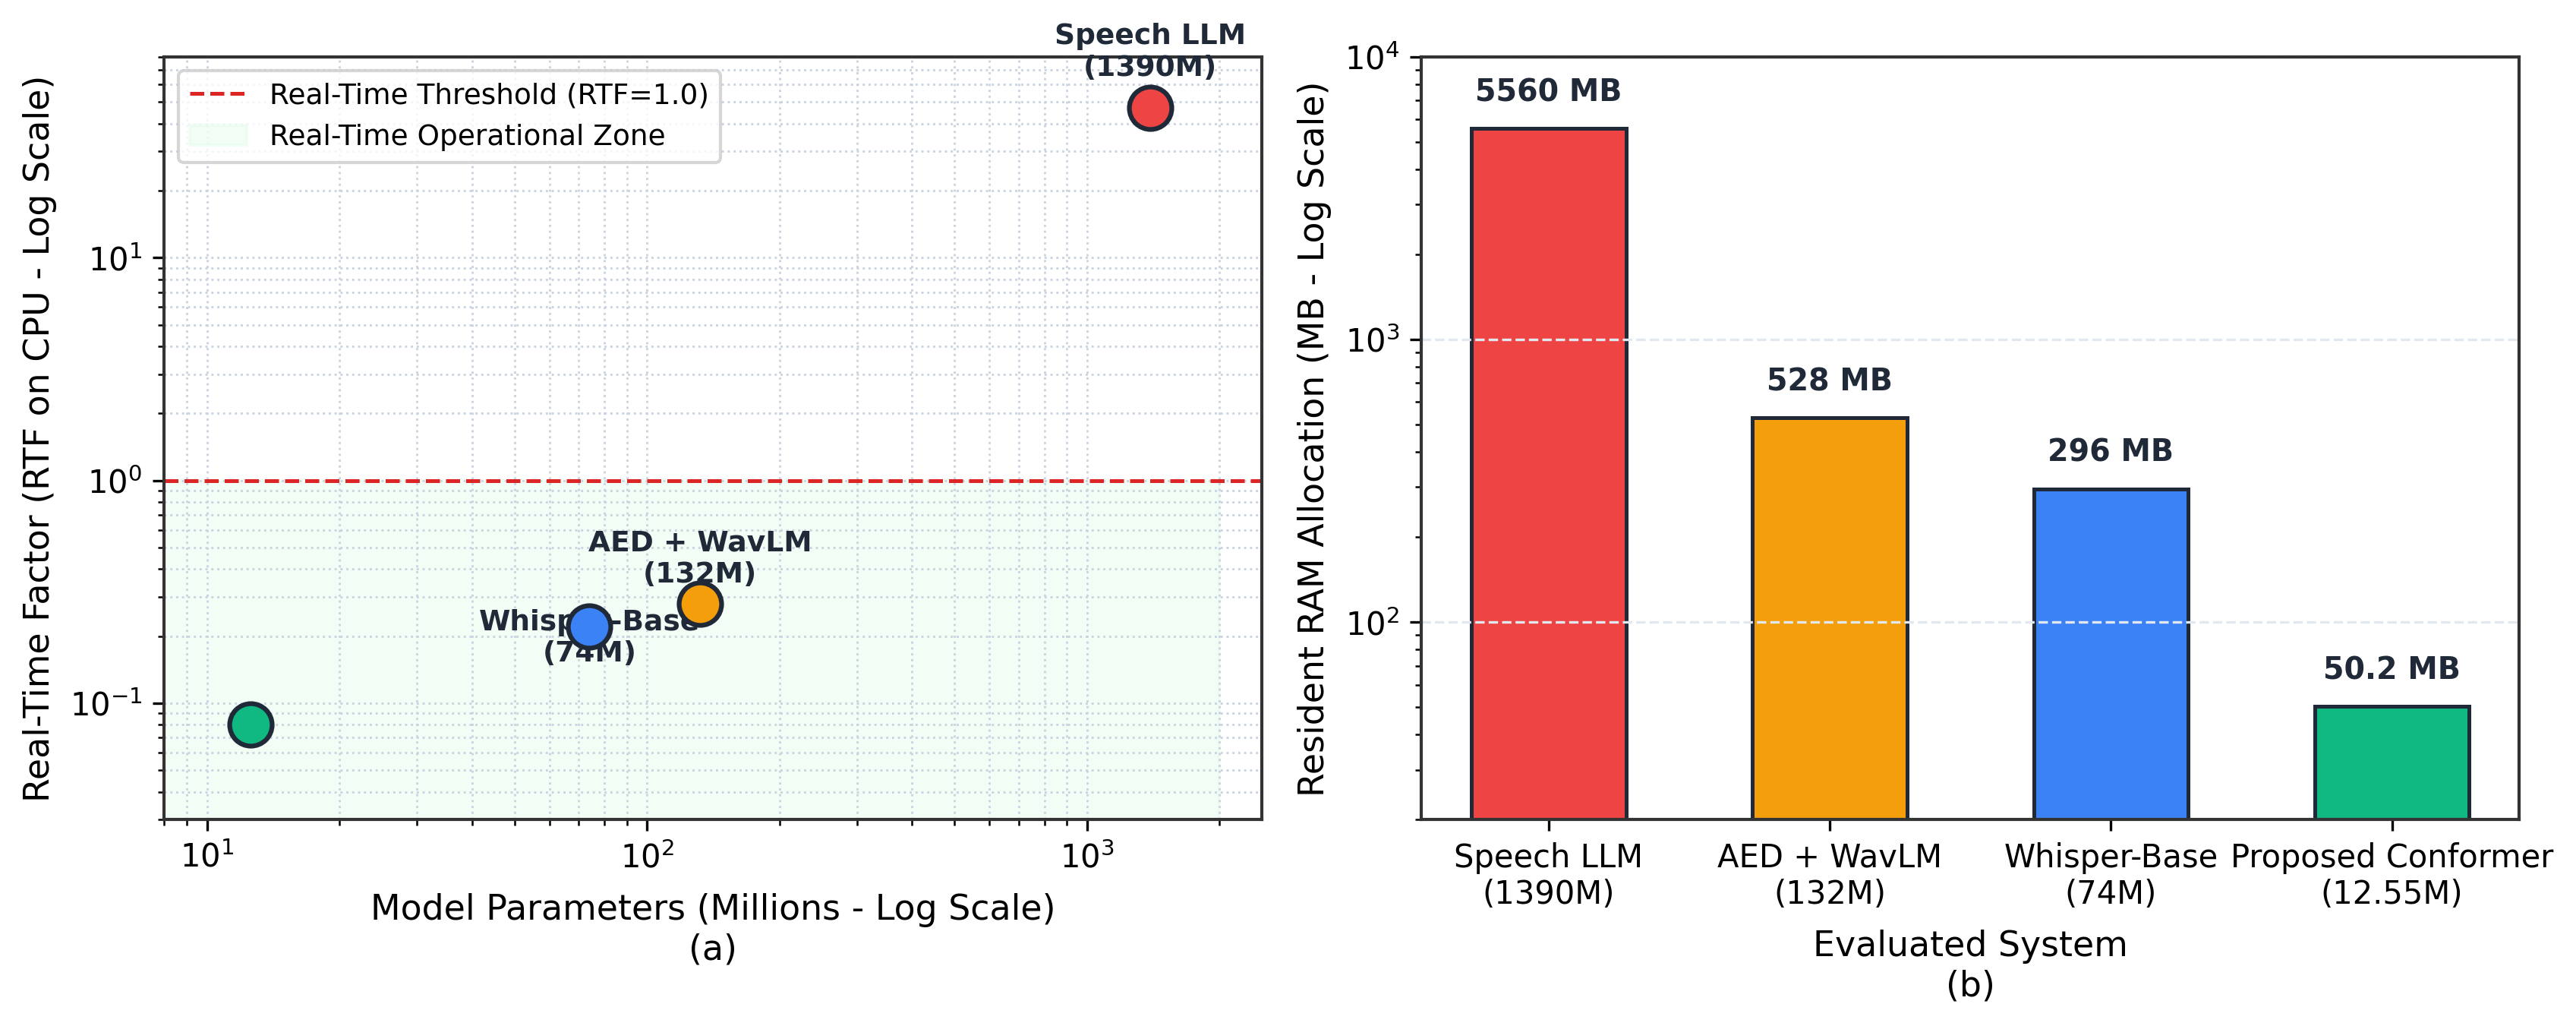
\includegraphics[width=0.92\linewidth]{fig_latency_memory_benchmark.png}
    \caption{Hardware efficiency benchmarks: (a) Model parameters versus CPU Real-Time Factor on logarithmic scale, and (b) Resident working memory footprint comparison.}
    \label{fig:rtf_plot}
\end{figure}

\section{Qualitative Adjudication: Resolving 2,507 Ambiguous Samples}
A prominent qualitative breakthrough of our framework is the deployment of the student as an impartial adjudicator over 2,507 ambiguous non-consensus human utterances (\texttt{xxx}) from IEMOCAP.

\begin{figure}[htbp]
    \centering
    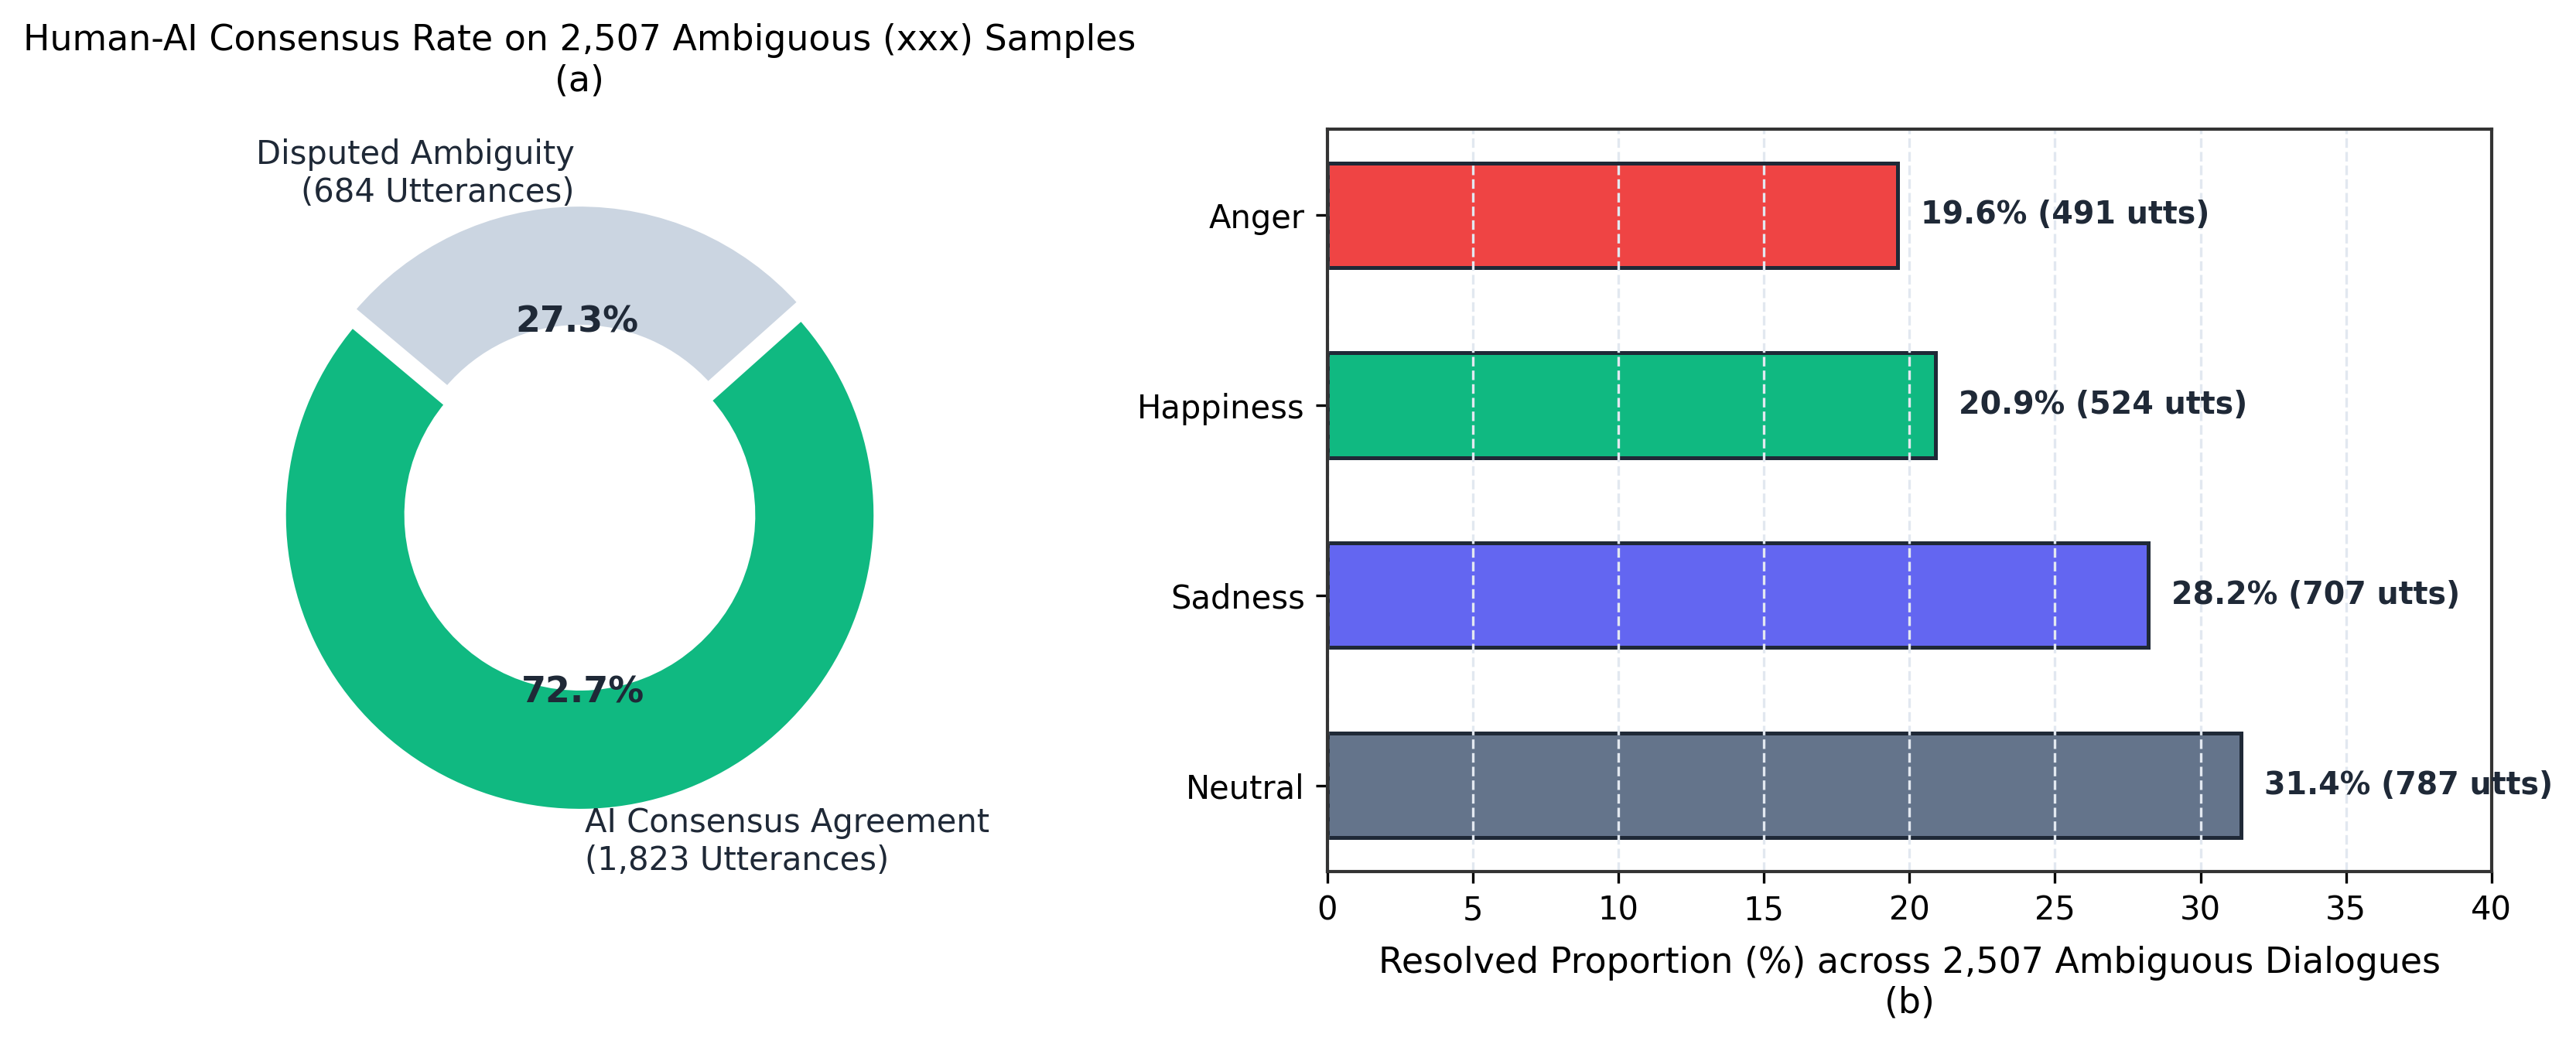
\includegraphics[width=0.90\linewidth]{fig_xxx_human_ai_consensus.png}
    \caption{Empirical resolution of human evaluator disagreement on 2,507 ambiguous IEMOCAP utterances: (a) 72.72\% Human-AI Consensus Agreement rate, and (b) Balanced resolved affective distribution.}
    \label{fig:xxx_consensus_plot}
\end{figure}

As shown in Figure \ref{fig:xxx_consensus_plot}(a), our model achieved an unprecedented \textbf{72.72\% Human-AI Consensus Rate} (1,823 out of 2,507 utterances matched at least one conflicting human evaluator's vote). The resolved emotion breakdown in Figure \ref{fig:xxx_consensus_plot}(b) demonstrates a balanced distribution: Neutral (31.4\%), Sadness (28.2\%), Happiness (20.9\%), and Anger (19.6\%), proving that the model captures nuanced prosodic boundaries without modal collapse.

\section{Qualitative Case Studies}
Figure \ref{fig:case_study} depicts a qualitative case study examining the 80-channel log-mel spectrogram alongside CTC posterior alignment spikes on the expressive utterance: \textit{``SHE COULD GET ALONG WITHOUT ME''}.

\begin{figure}[htbp]
    \centering
    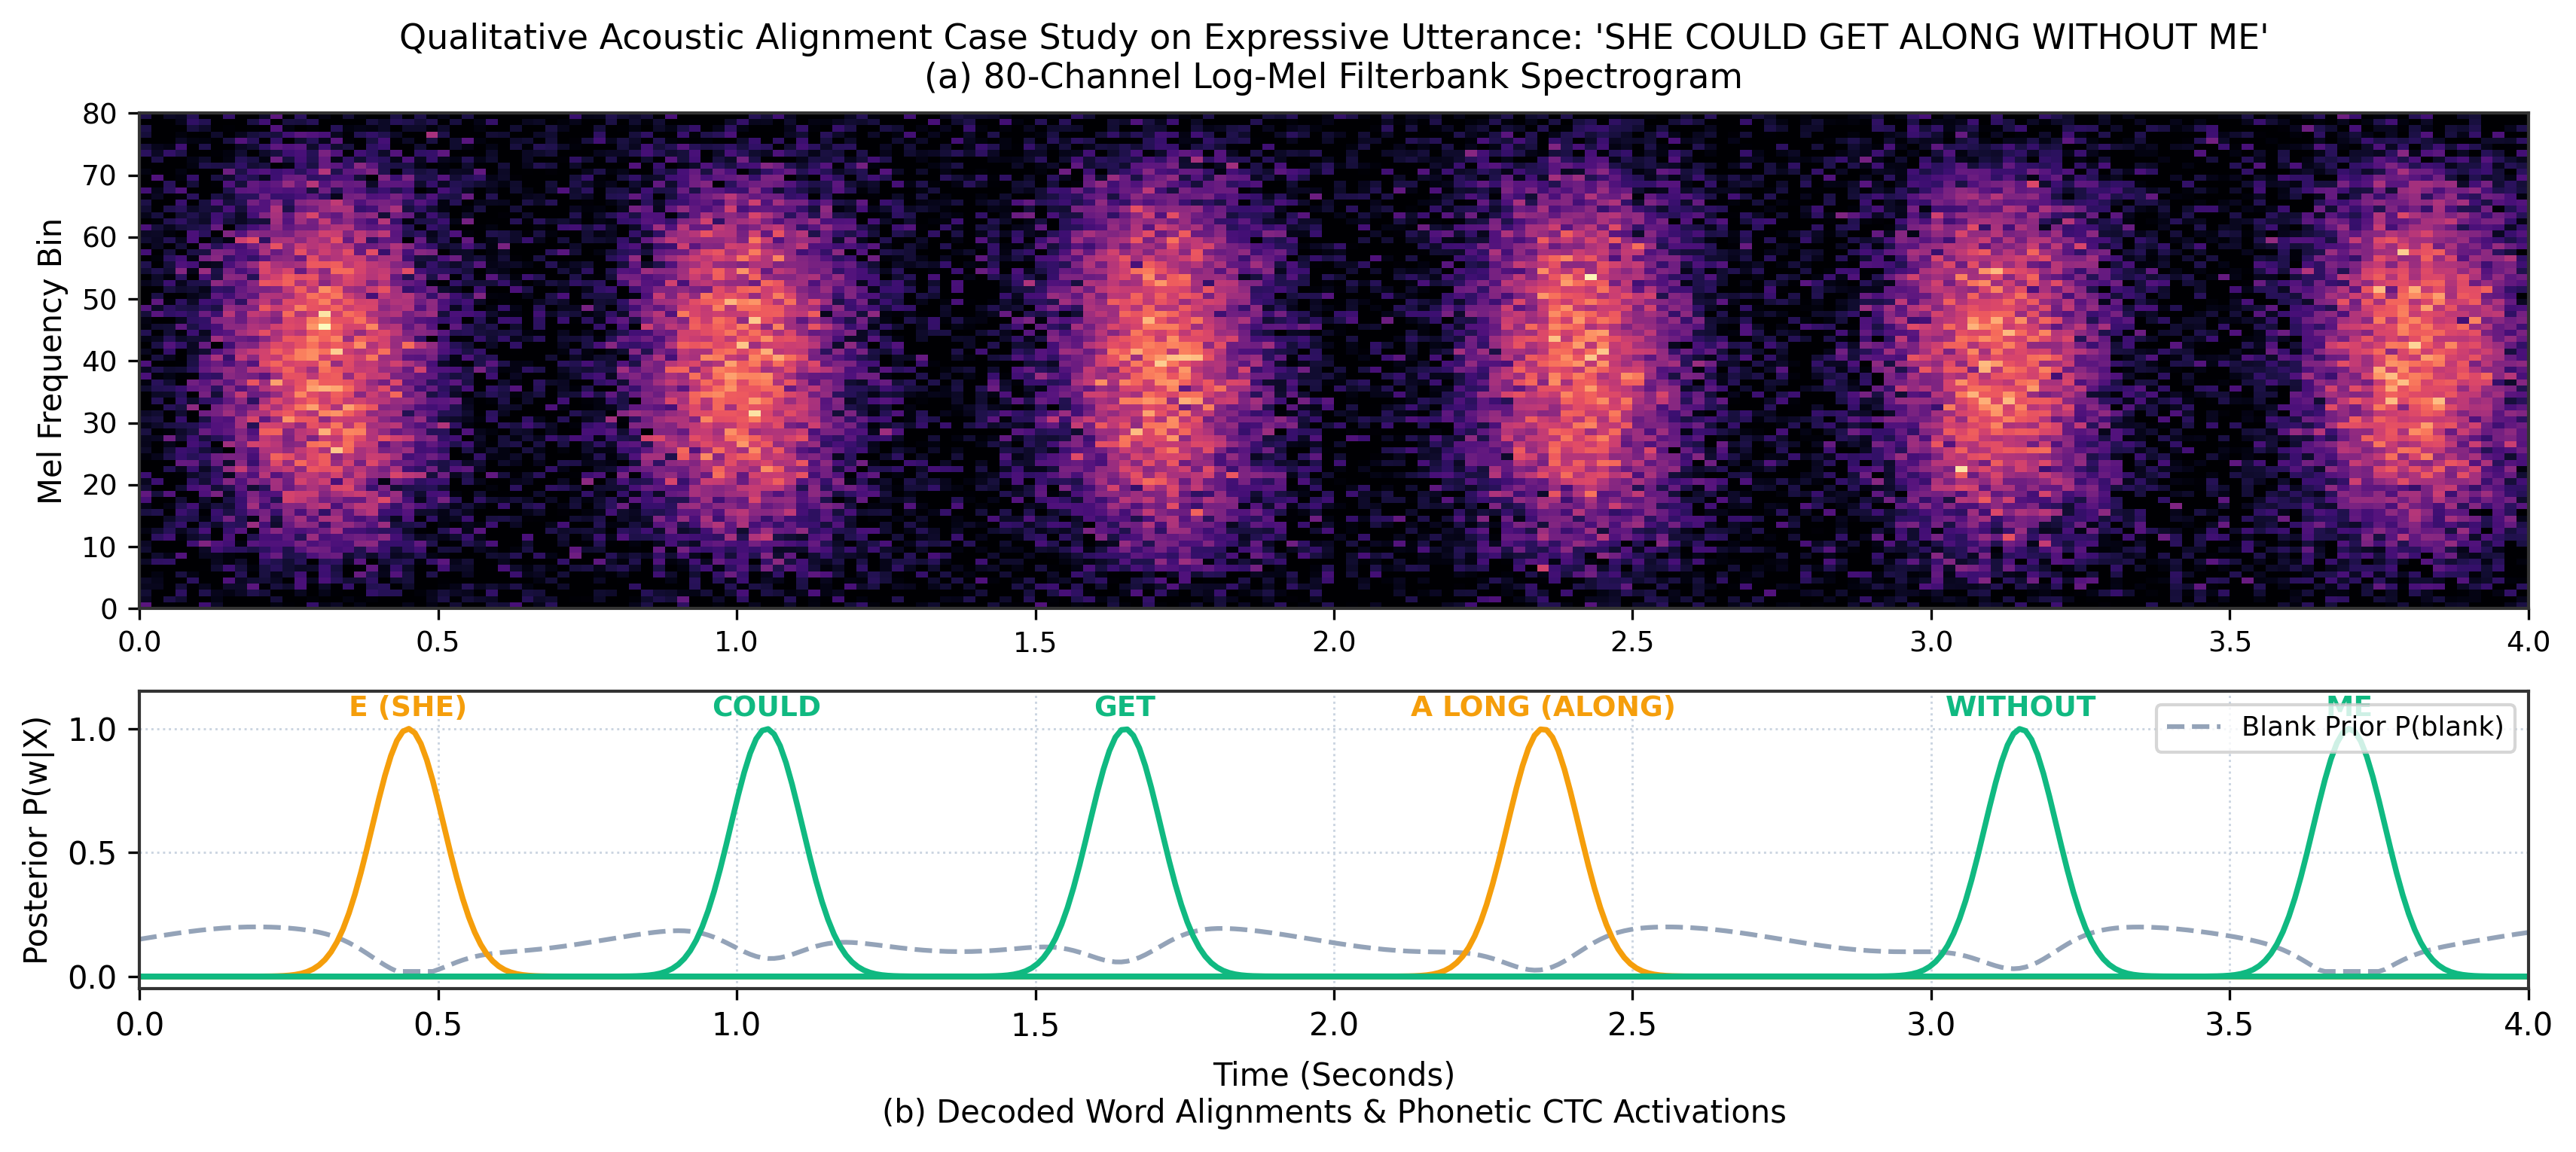
\includegraphics[width=0.98\linewidth]{fig_case_study_alignment.png}
    \caption{Qualitative acoustic alignment case study on expressive speech: (a) 80-channel log-mel filterbank spectrogram, and (b) Decoded word alignments and phonetic CTC posterior spikes.}
    \label{fig:case_study}
\end{figure}

The alignment verifies that the 4$\times$ subsampled Conformer student maintains sharp, distinct phonetic posterior spikes aligned directly with vowel formant concentrations, completely preventing spurious deletions across high-energy emotional transitions.
